\chapter{Wizualizacja procesu}
\label{inteco_wizualizacja}

\section{Reprezentacja graficzna procesu}
\label{inteco_wizualizacja_repr}
Tworzenie panelu operatorskiego rozpoczęliśmy od utworzenia ekranu zawierającego wizualizację procesu. Na ekranie możemy obserwować wartości sygnałów procesowych dla każdego toru regulacji. Ekran zawiera wartości wyjść, sterowań oraz wartości zadanych. Na ekranie możemy również obserwować uproszczony rysunek sterowanego obiektu.
\\

\begin{figure}[H]
    \label{TCRANE::Wizualizacja}
    \centering
    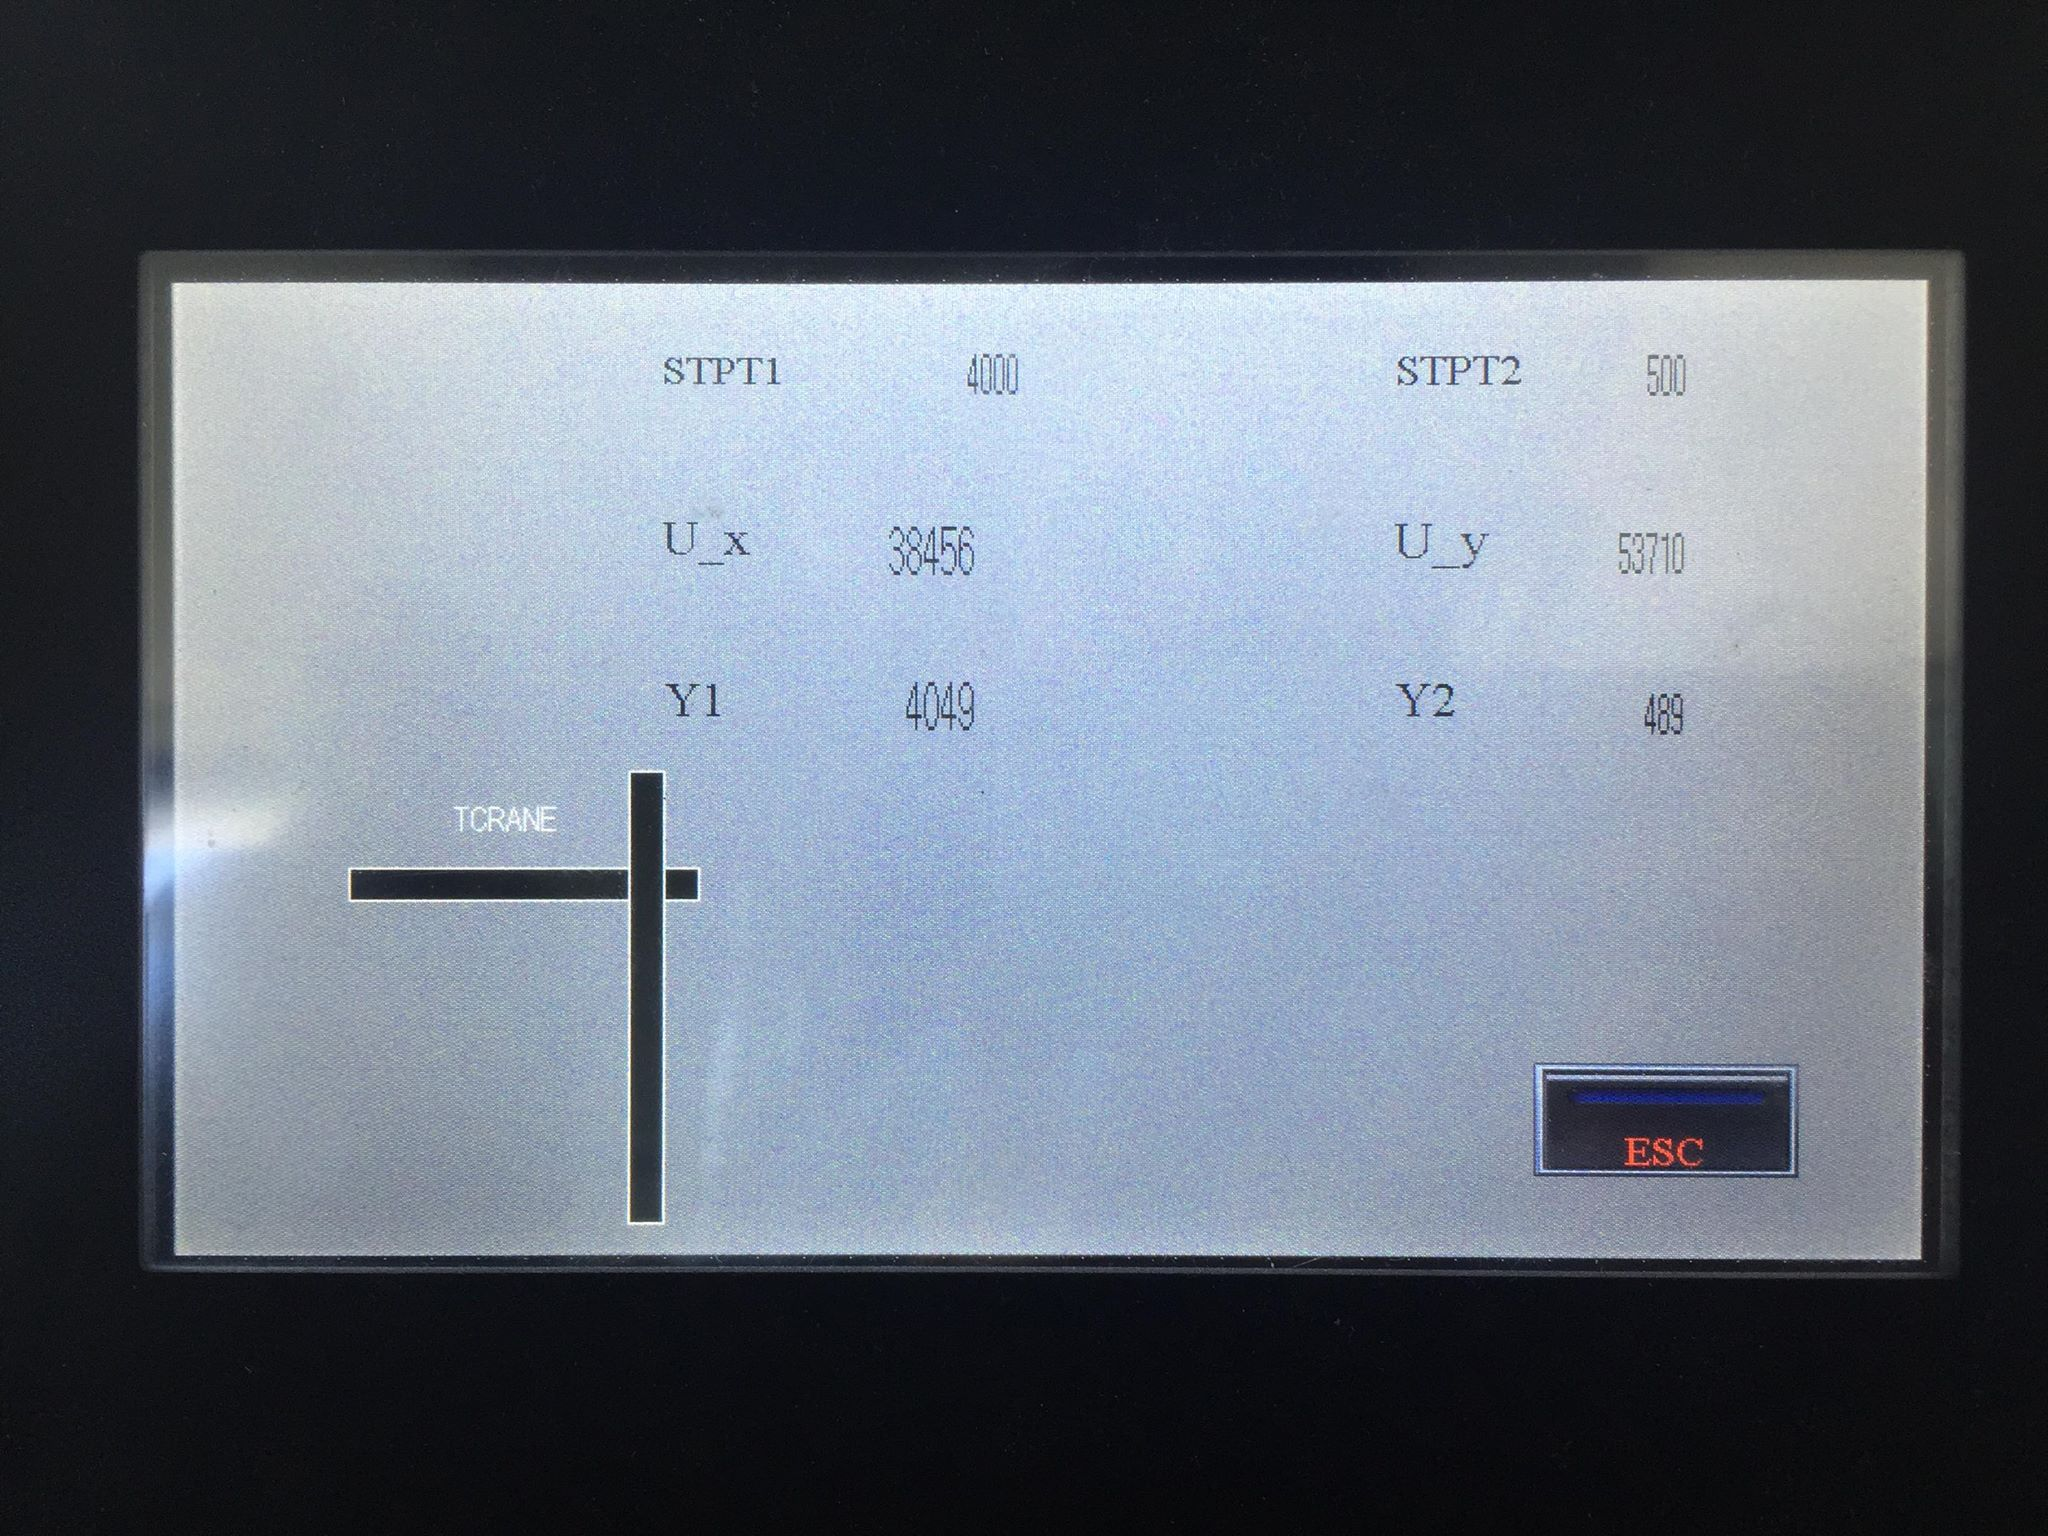
\includegraphics[scale=0.15]{./sections/inteco/images/reprezentacja_obiektu.jpg}
    \caption{Wizualizacja procesu}
\end{figure}

\section{Prezentacja sygnałów regulacji}
\label{inteco_wizualizacja_wykresy}
W procesie tworzenia panelu operatorskiego zawierało się również utworzenie ekranów zawierających przebiegi sygnałów procesowych. W celu umożliwienia wygodnej obserwacji sygnałów utworzone zostały cztery osobne ekrany zawierające wykresy sygnałów wyjść obiektu w osiach X oraz Y, a także wykresy sterowań dla każdego wyjścia.

\begin{figure}[H]
    \label{Wykresy::output_x}
    \centering
    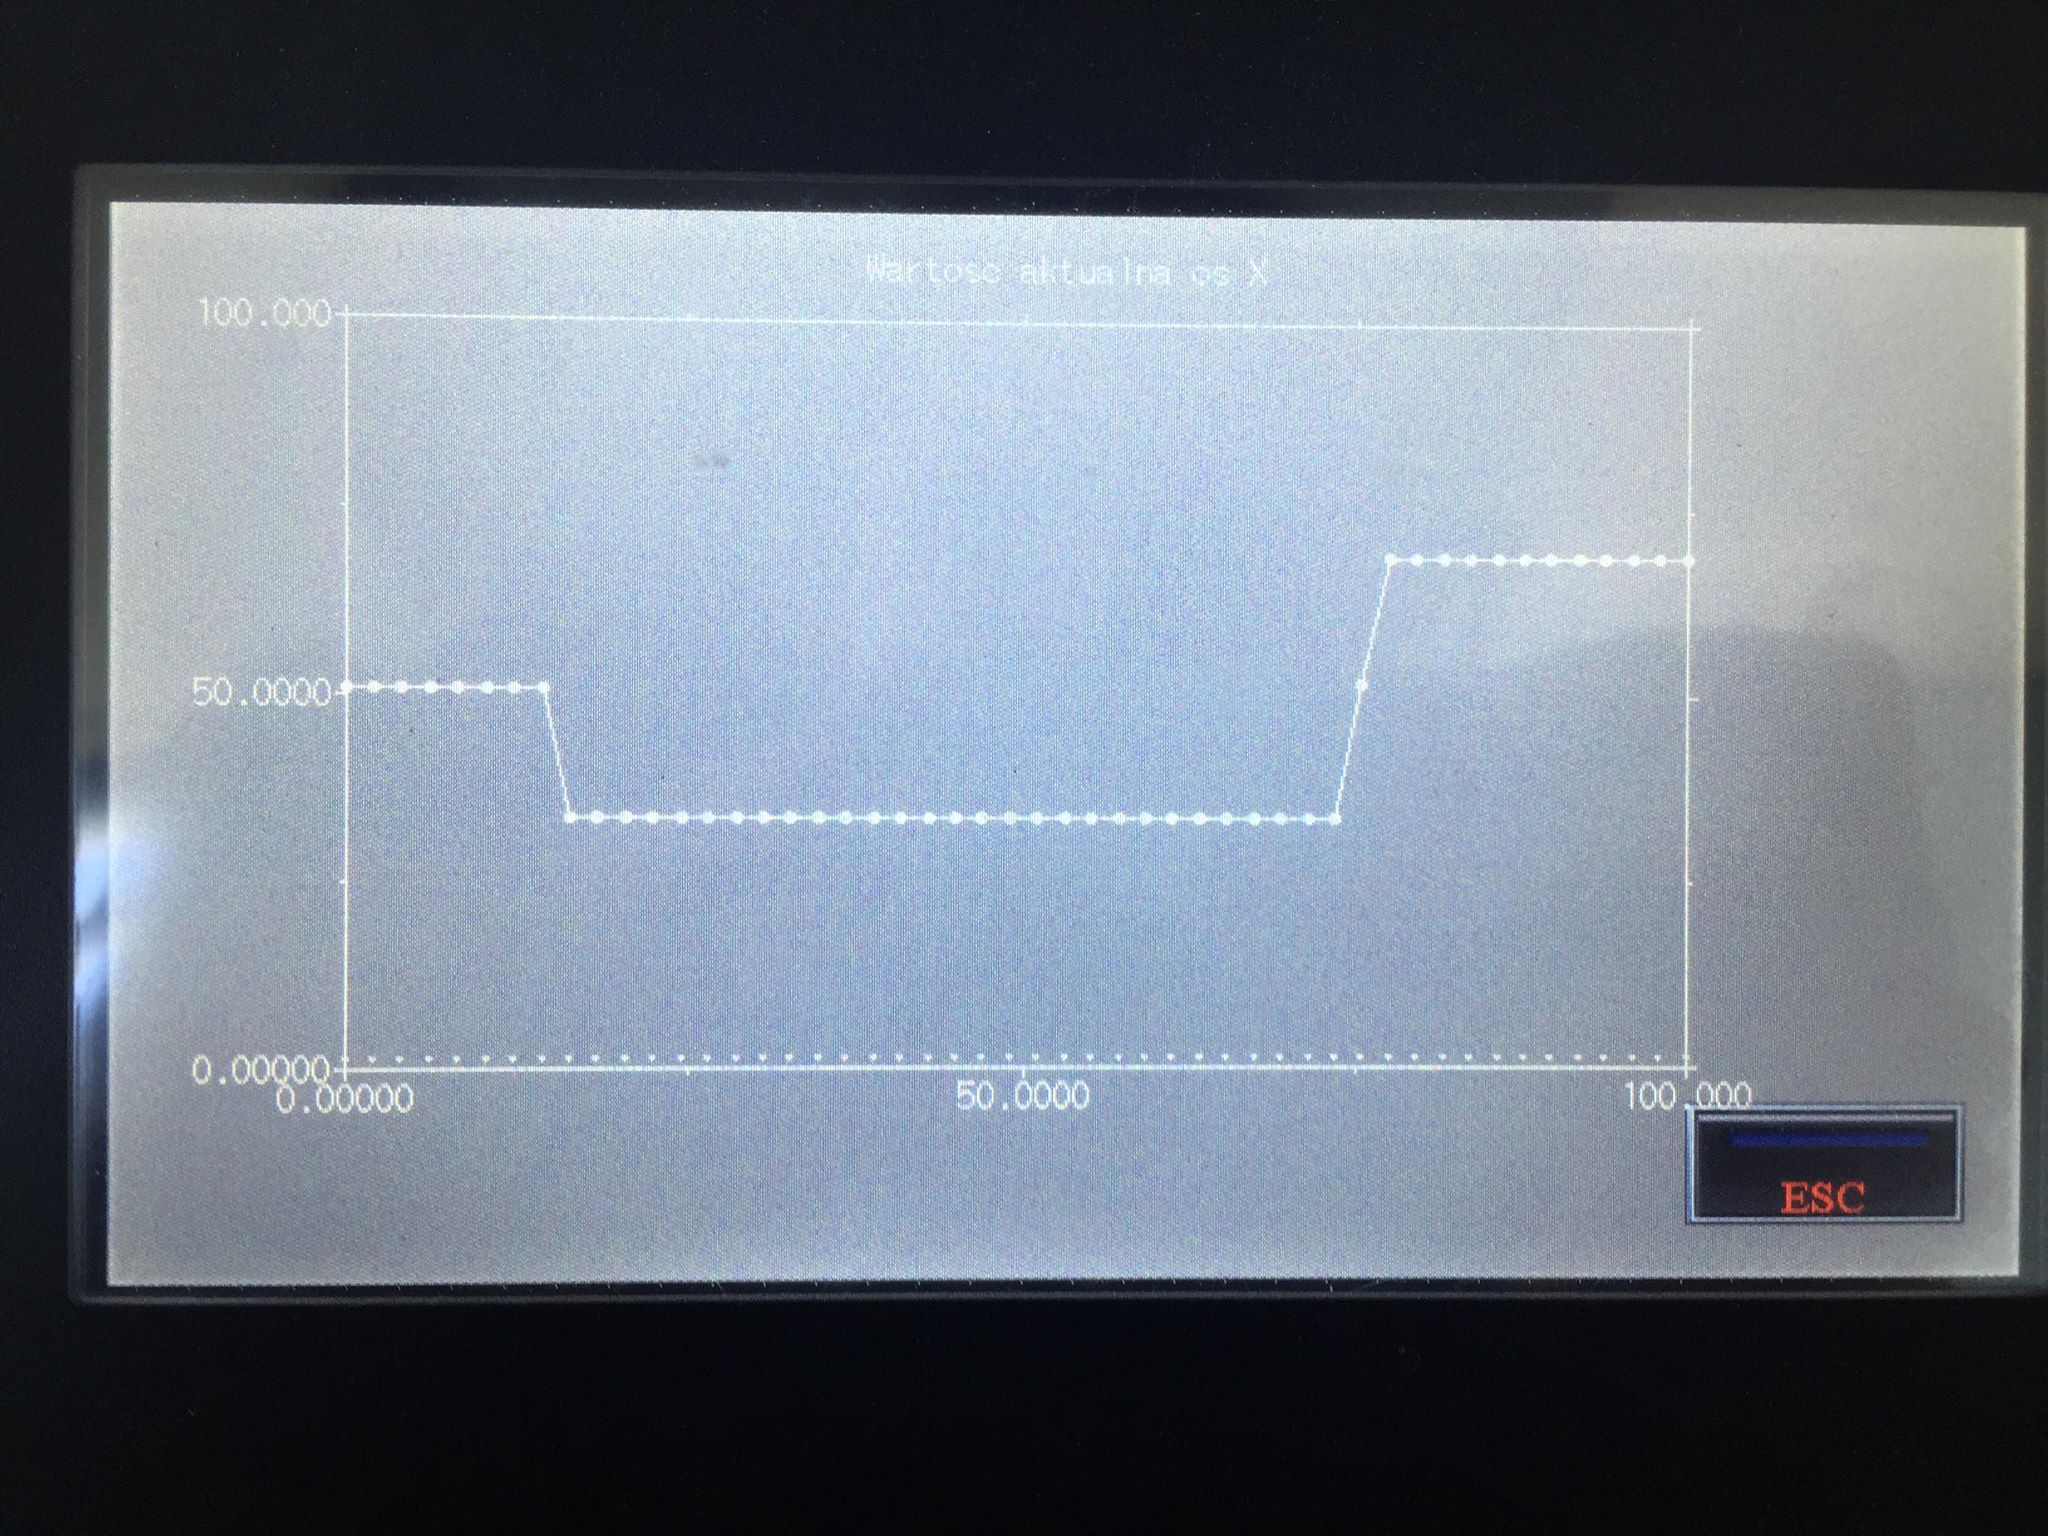
\includegraphics[scale=0.15]{./sections/inteco/images/output_x.jpg}
    \caption{Przebieg wyjścia dla osi X}
\end{figure}

\begin{figure}[H]
    \label{Wykres::input_x}
    \centering
    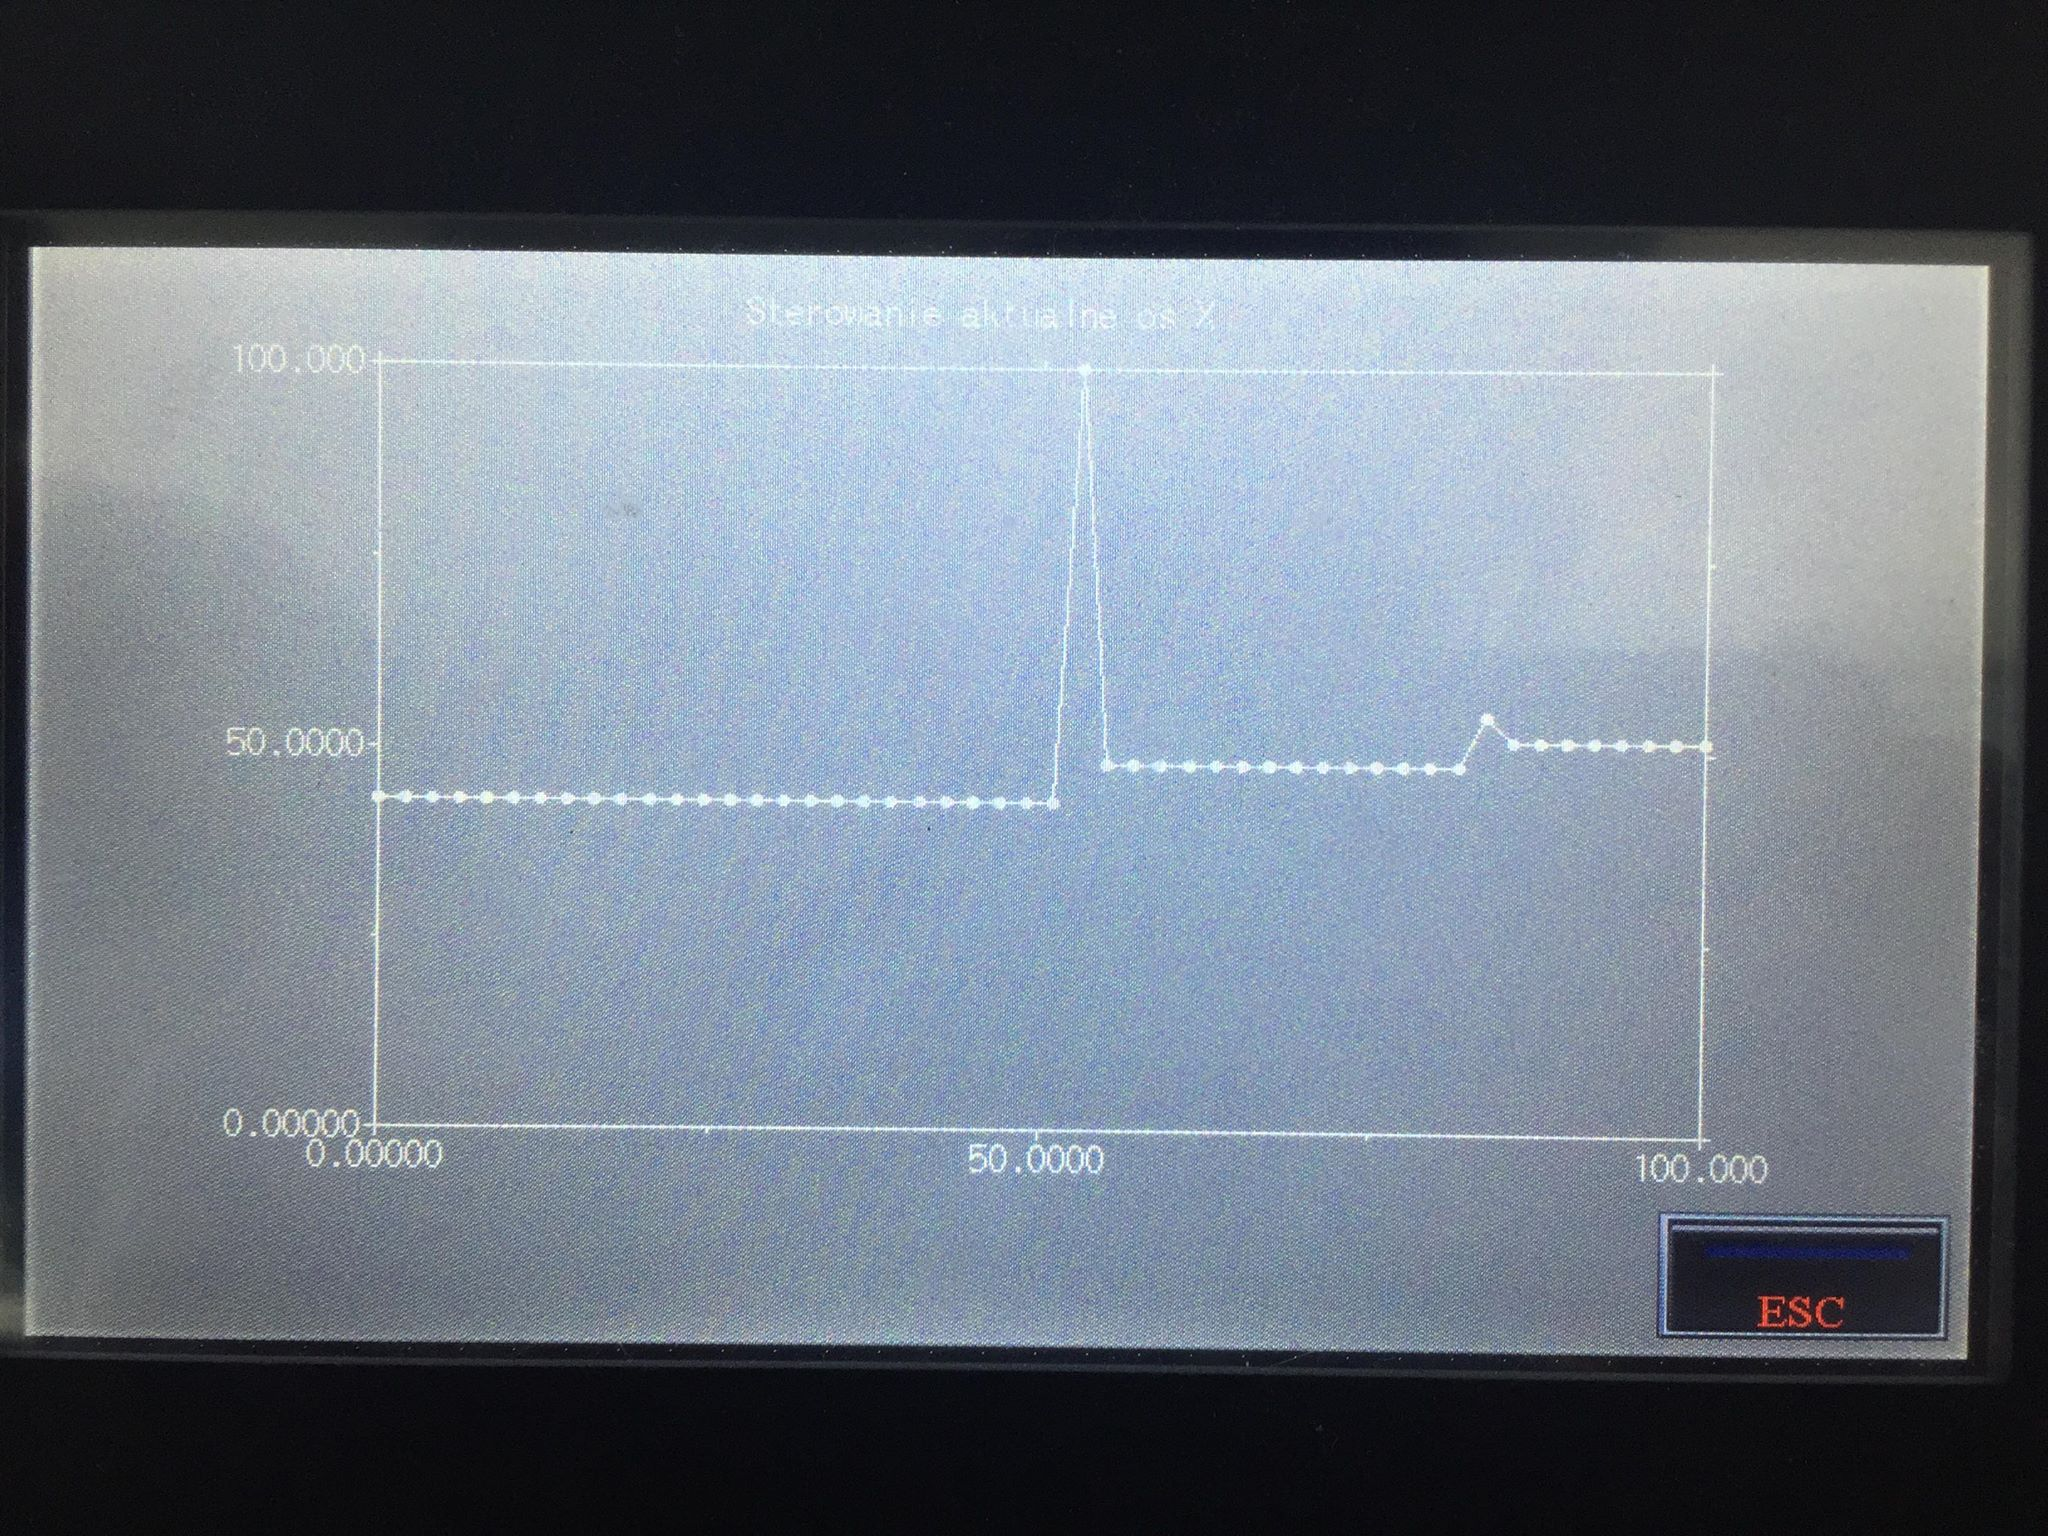
\includegraphics[scale=0.15]{./sections/inteco/images/input_x.jpg}
    \caption{Sterowanie dla osi X}
\end{figure}

\begin{figure}[H]
    \label{Wykres::output_y}
    \centering
    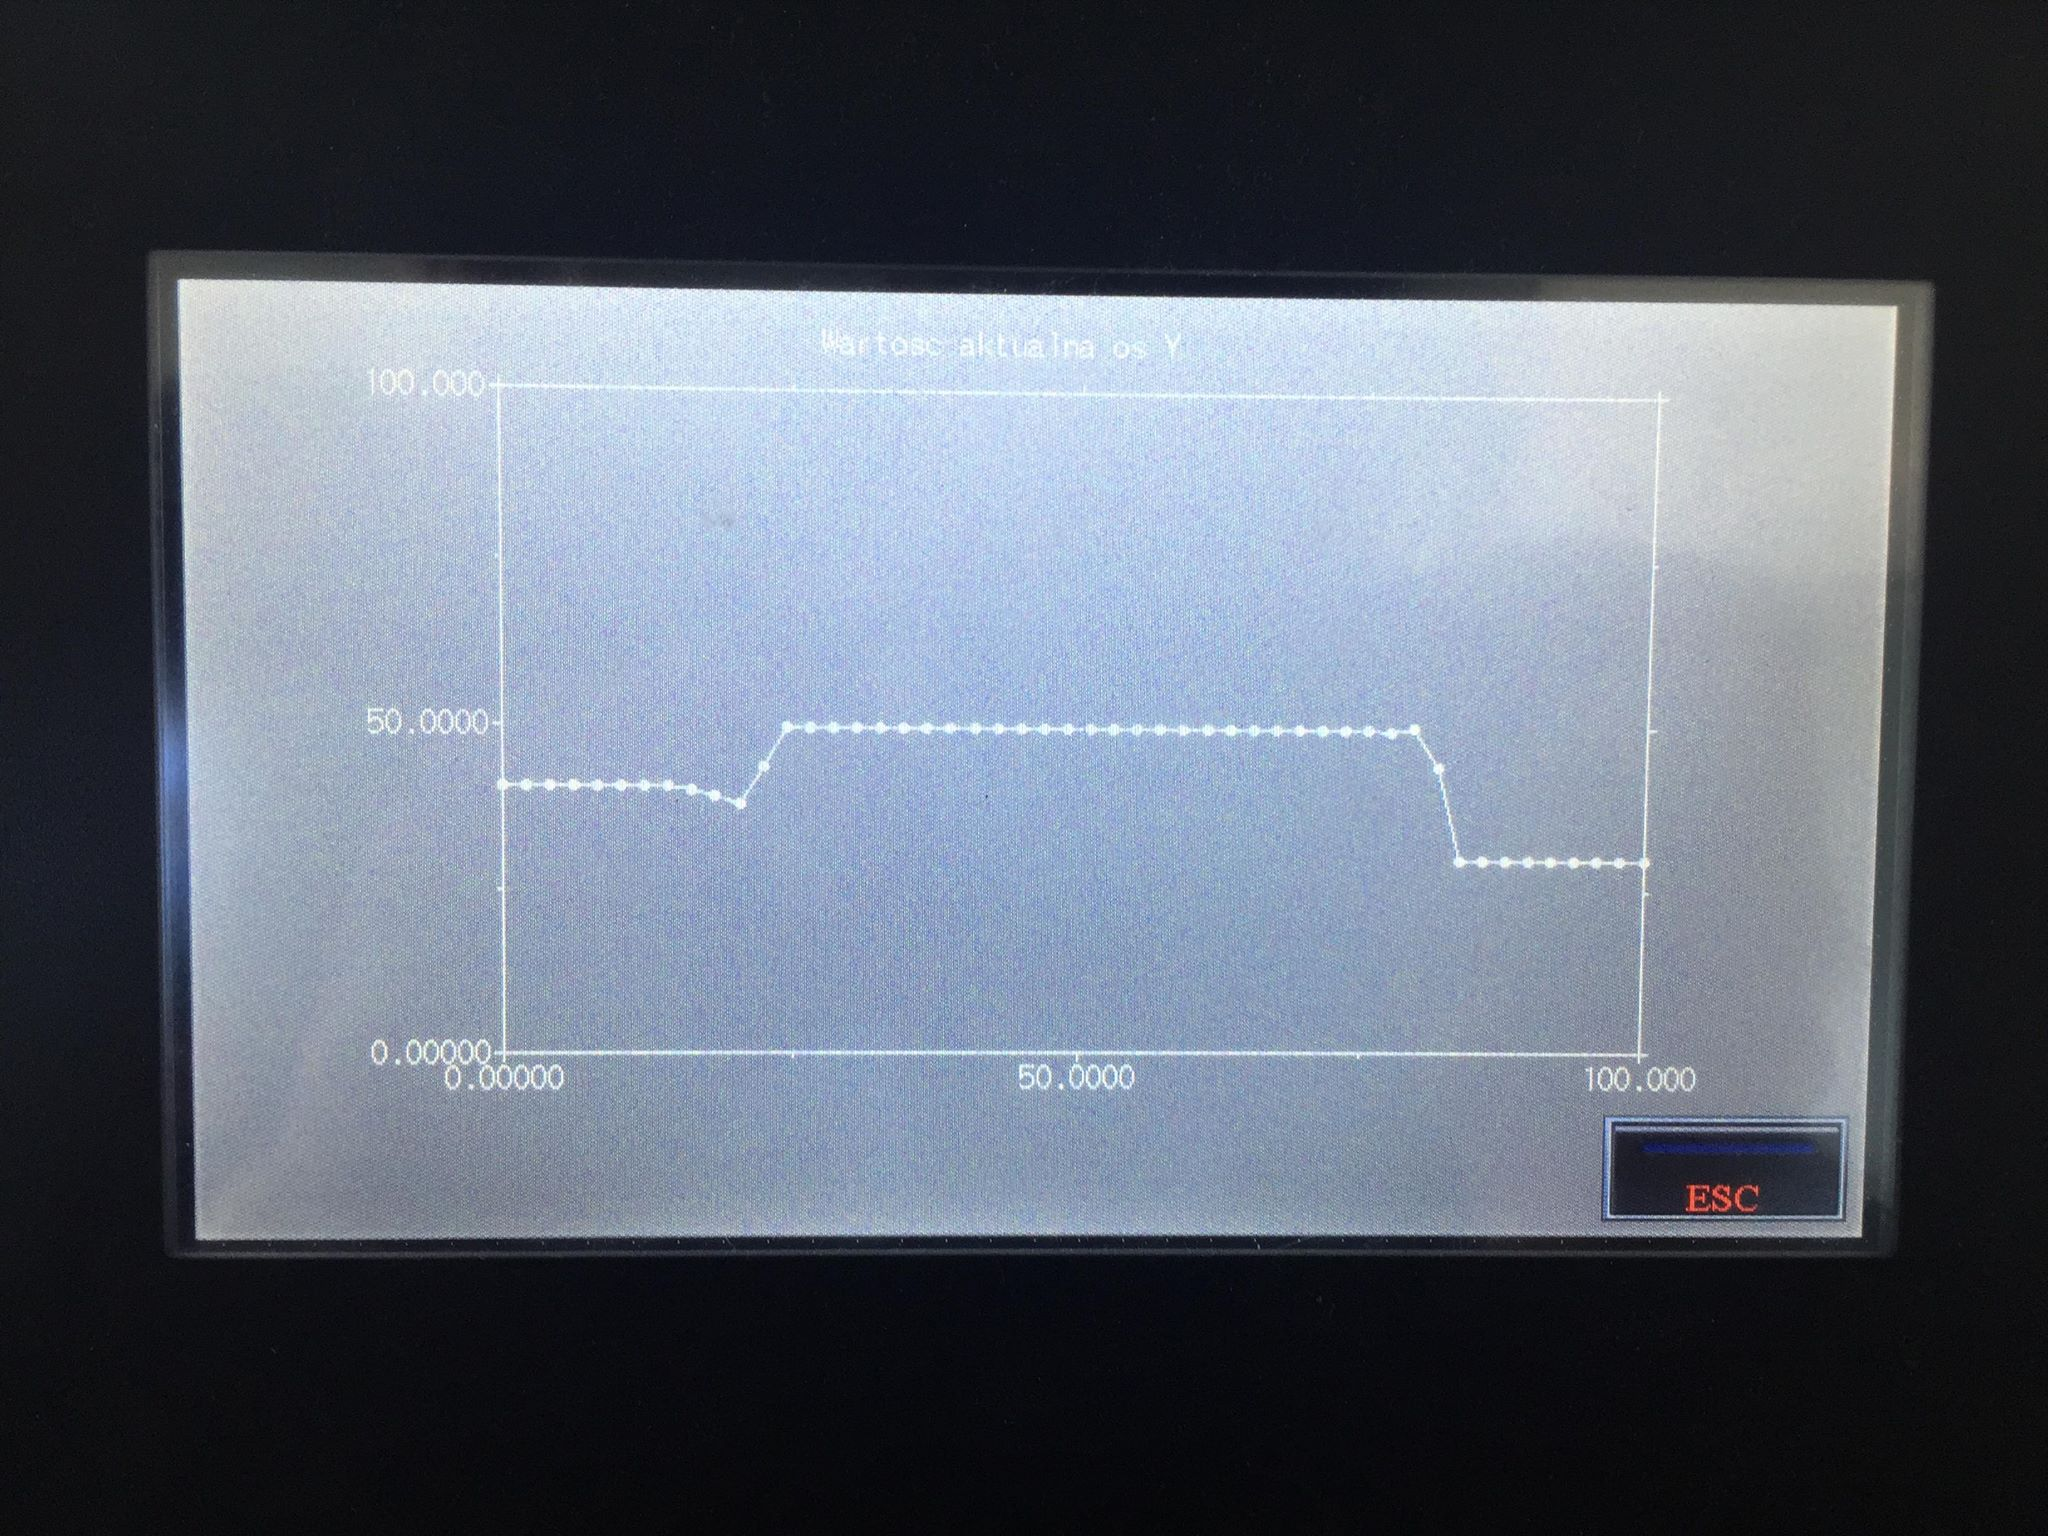
\includegraphics[scale=0.15]{./sections/inteco/images/output_y.jpg}
    \caption{Przebieg wyjścia dla osi Y}
\end{figure}

\begin{figure}[H]
    \label{Wykresy::input_y}
    \centering
    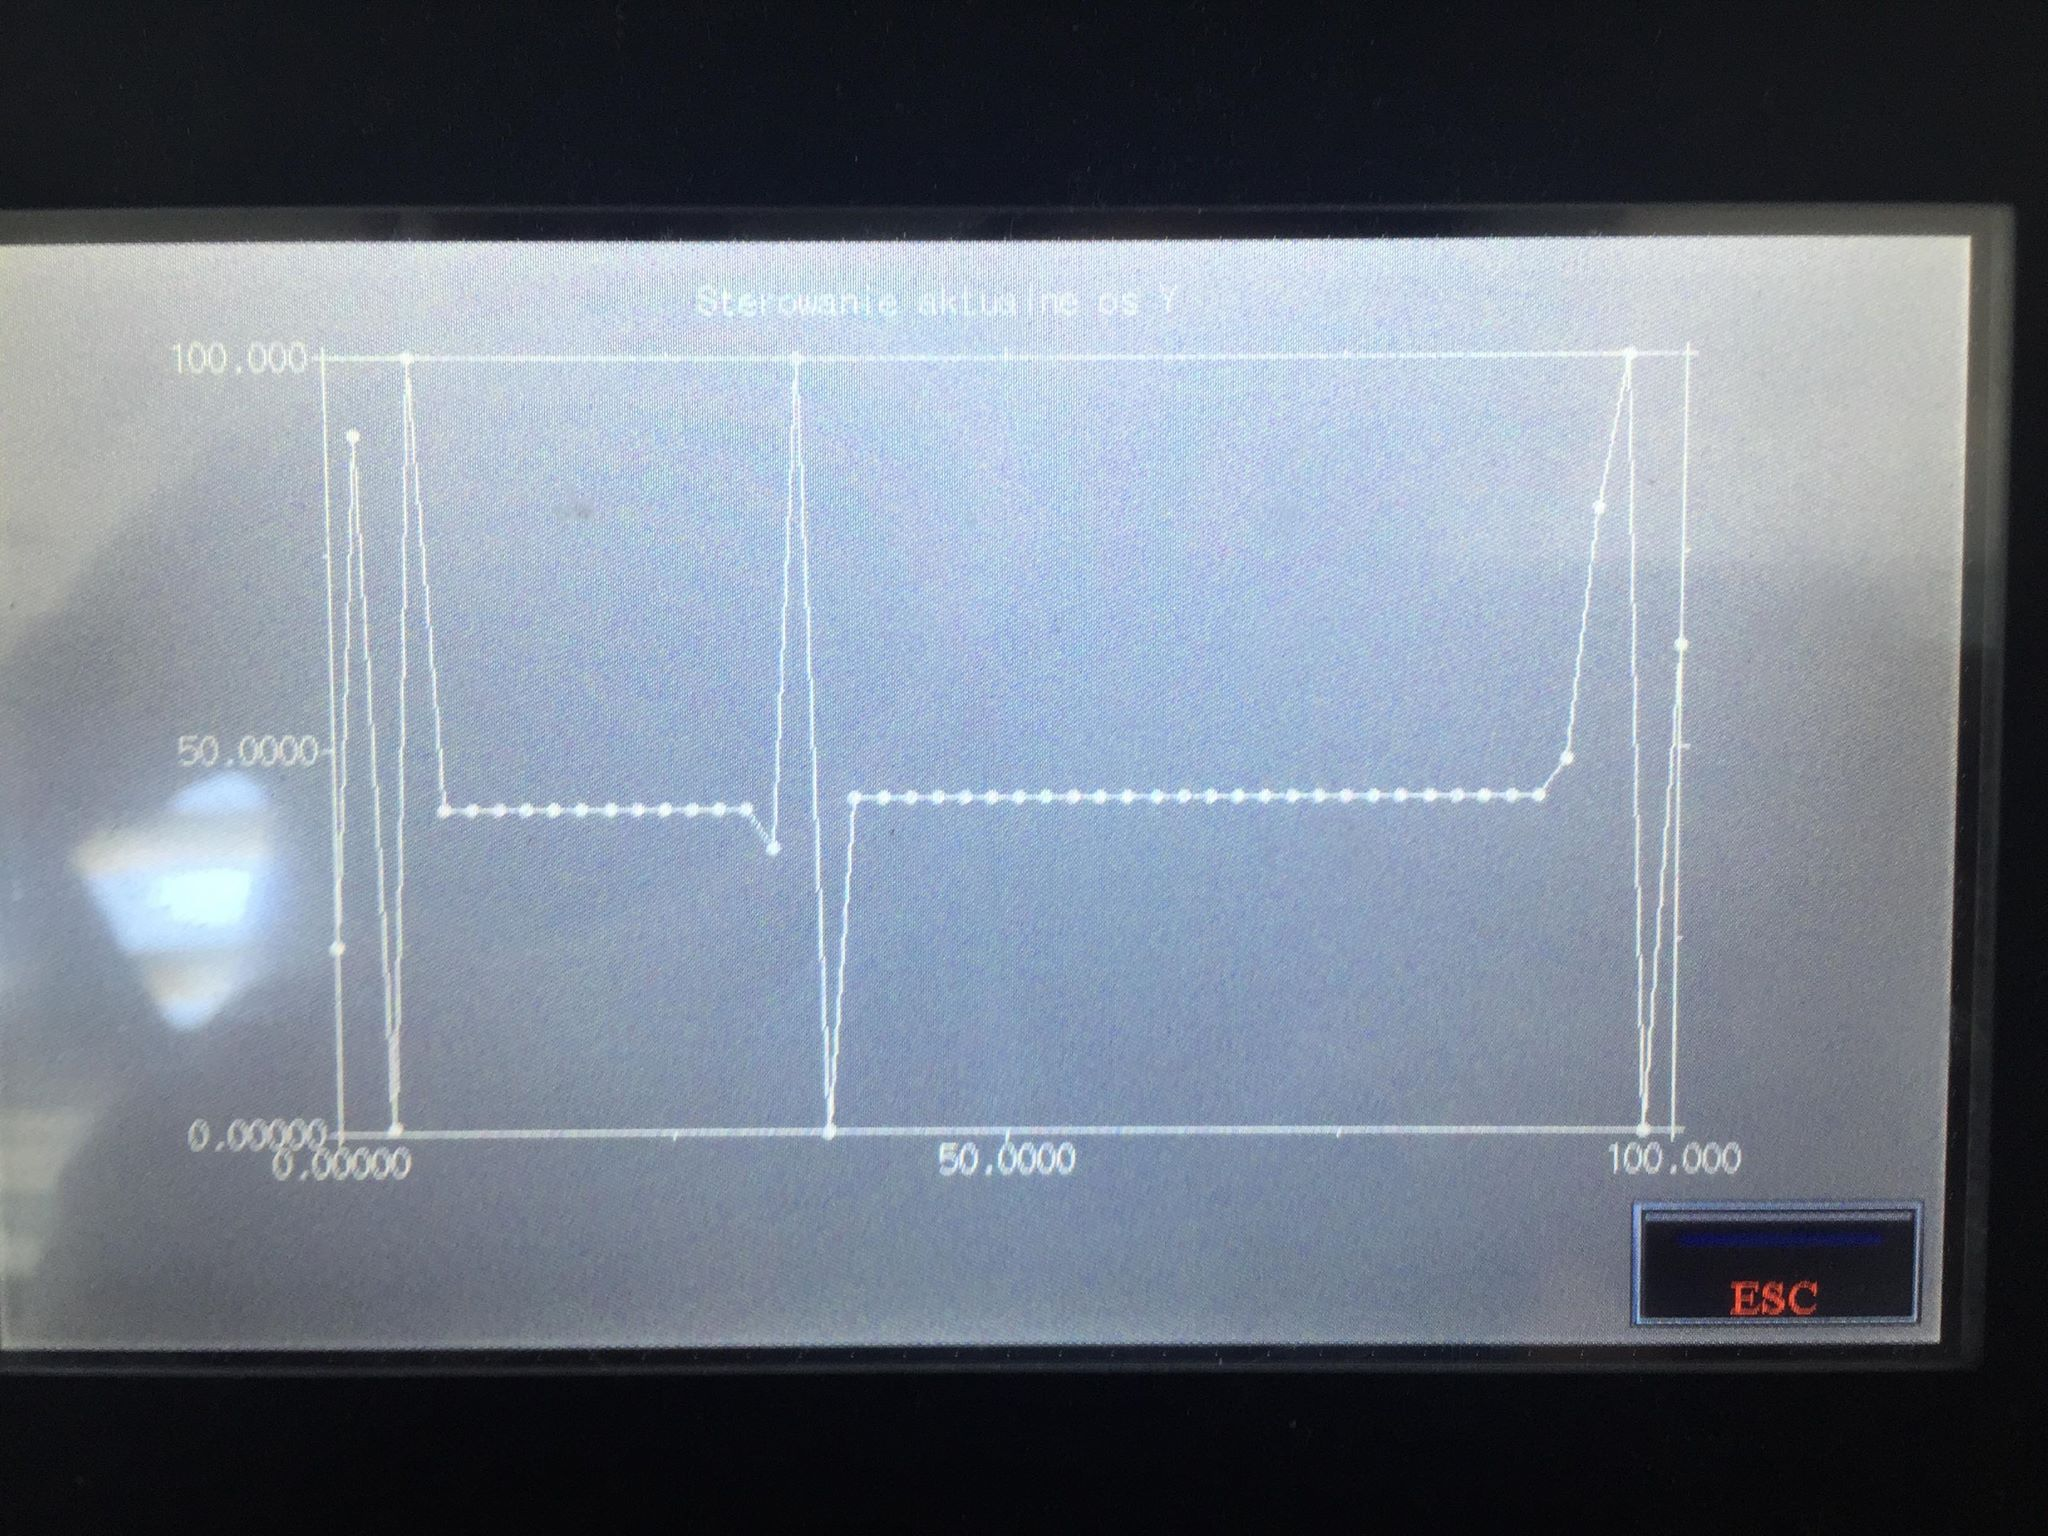
\includegraphics[scale=0.15]{./sections/inteco/images/input_y.jpg}
    \caption{Sterowanie dla osi Y}
\end{figure}

\section{Graf przejść automatu stanów}
\label{inteco_wizualizacja_automat}
W projekcie został również utworzony automat stanów procesu. Zmiany stanów następowały cyklicznie po upływie około 15 sekund. Ekran z automatem był zarówno ekranem początkowym, z którego można było przejść do każdego innego ekranu za pomocą przycisków znajdujących się po prawej stronie. Graf automatu znajduje się w centralnej części ekranu. Automat zawiera cztery stany. Dla stanu, w którym aktualnie znajduje się proces wyświetlany jest jego węzeł na grafie. Przykładowa prezentacja stanu procesu została przedstawiona na zdjęciach poniżej.

\begin{figure}[H]
    \label{automat_1}
    \centering
    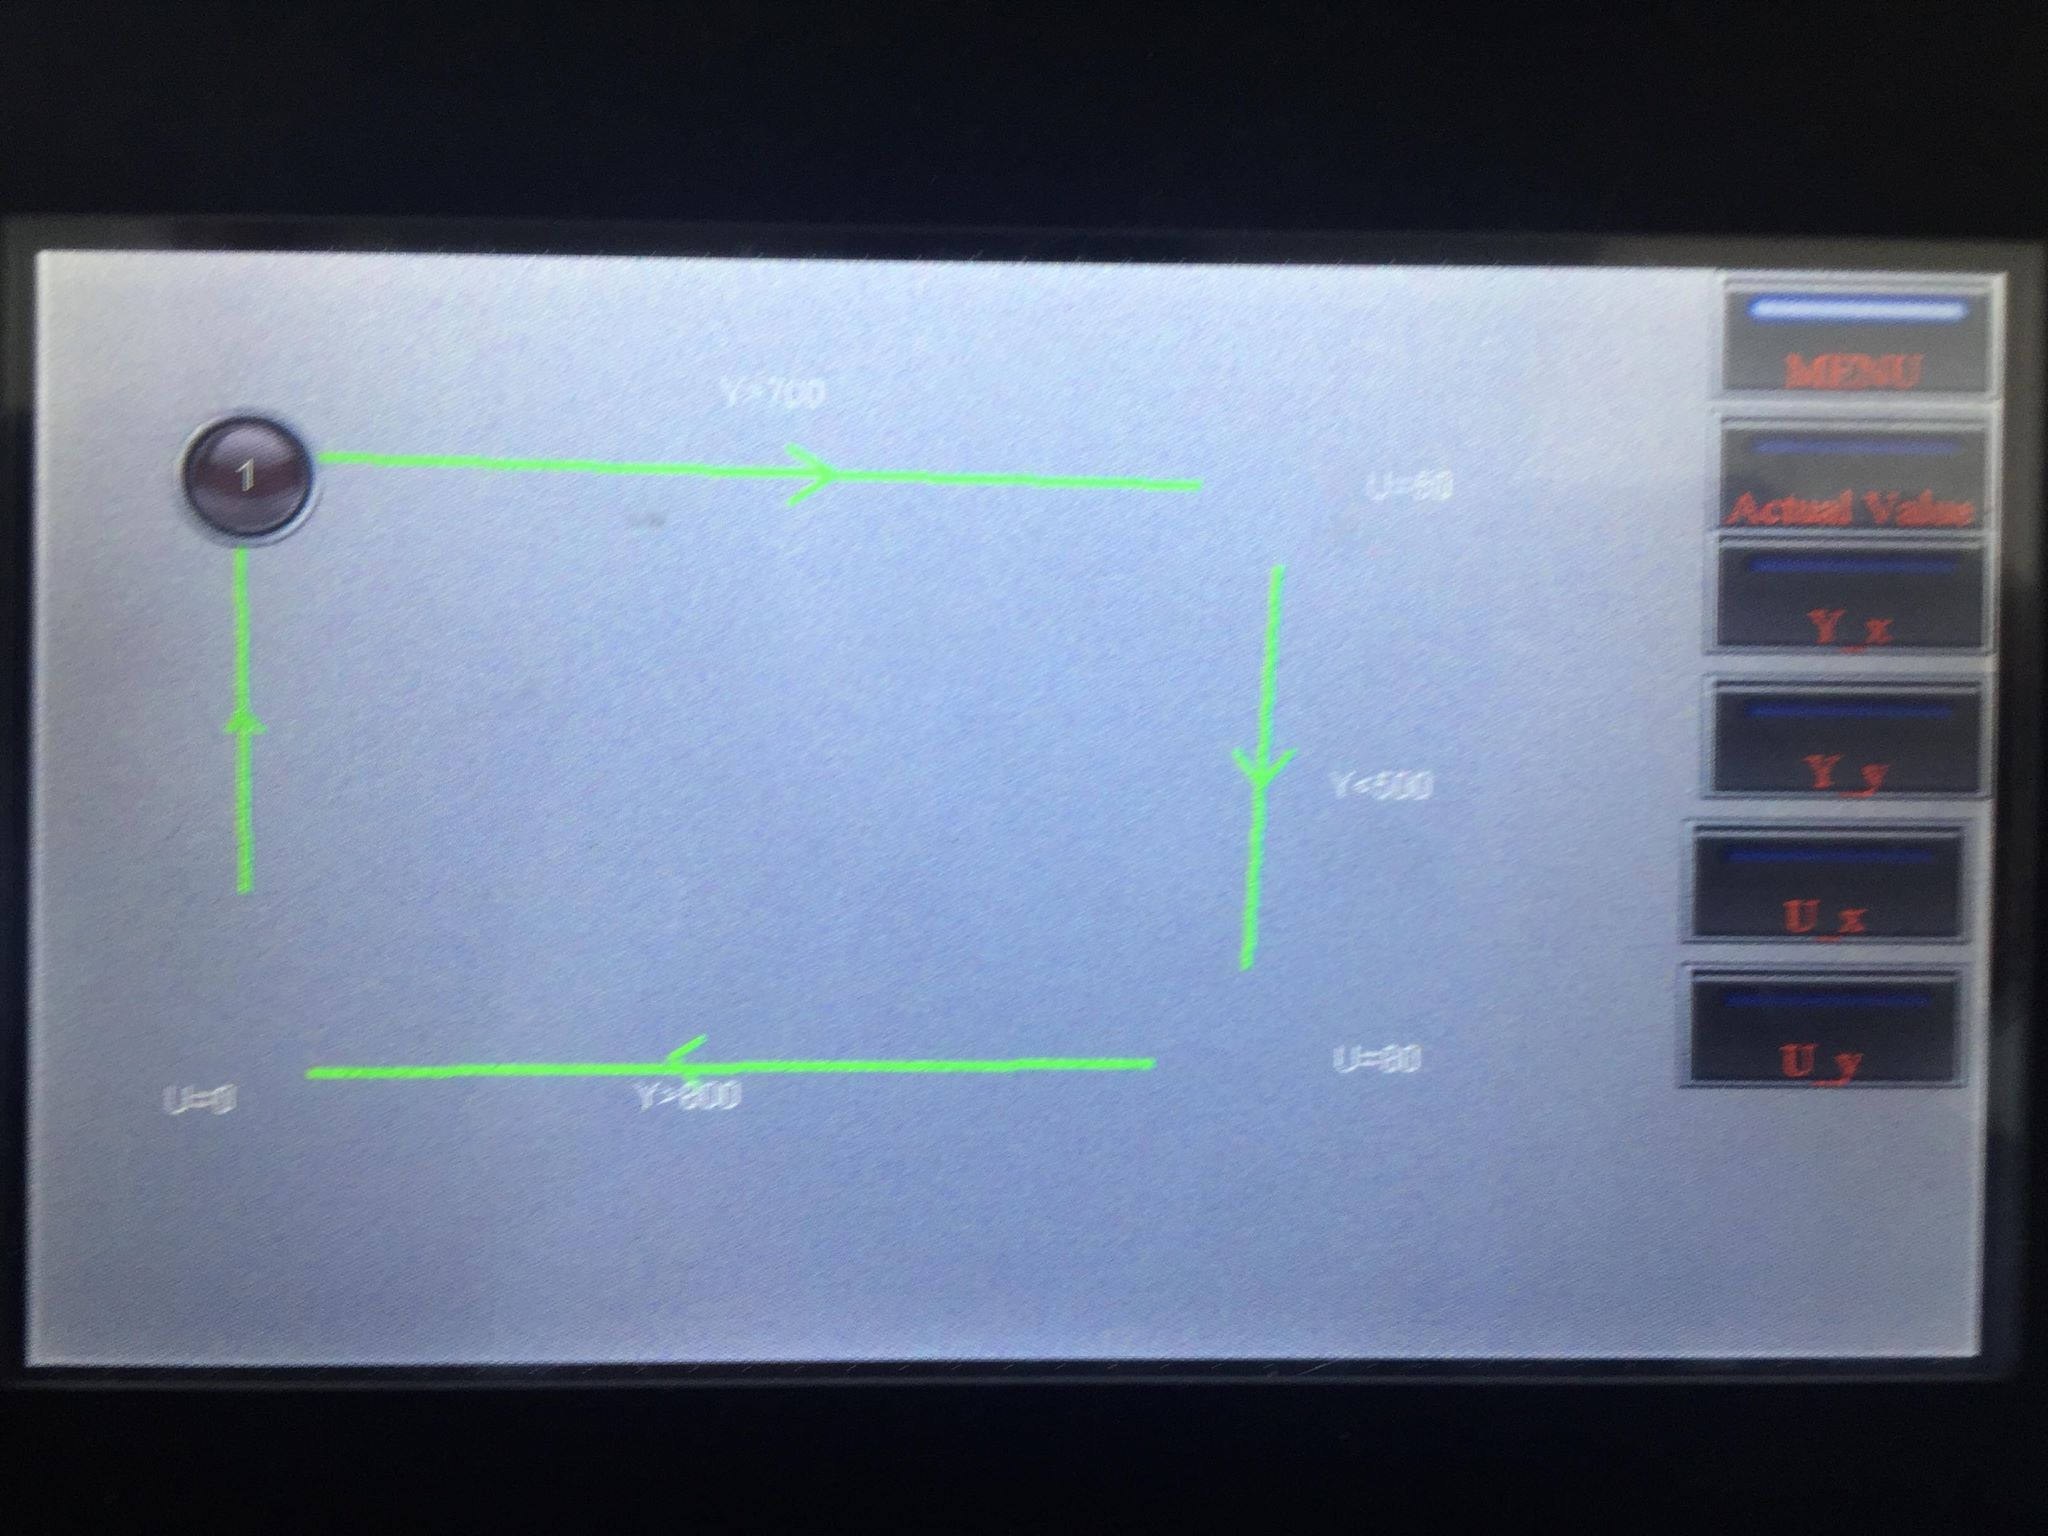
\includegraphics[scale=0.15]{./sections/inteco/images/automat1.jpg}
    \caption{Stan 1. procesu}
\end{figure}

\begin{figure}[H]
    \label{automat_3}
    \centering
    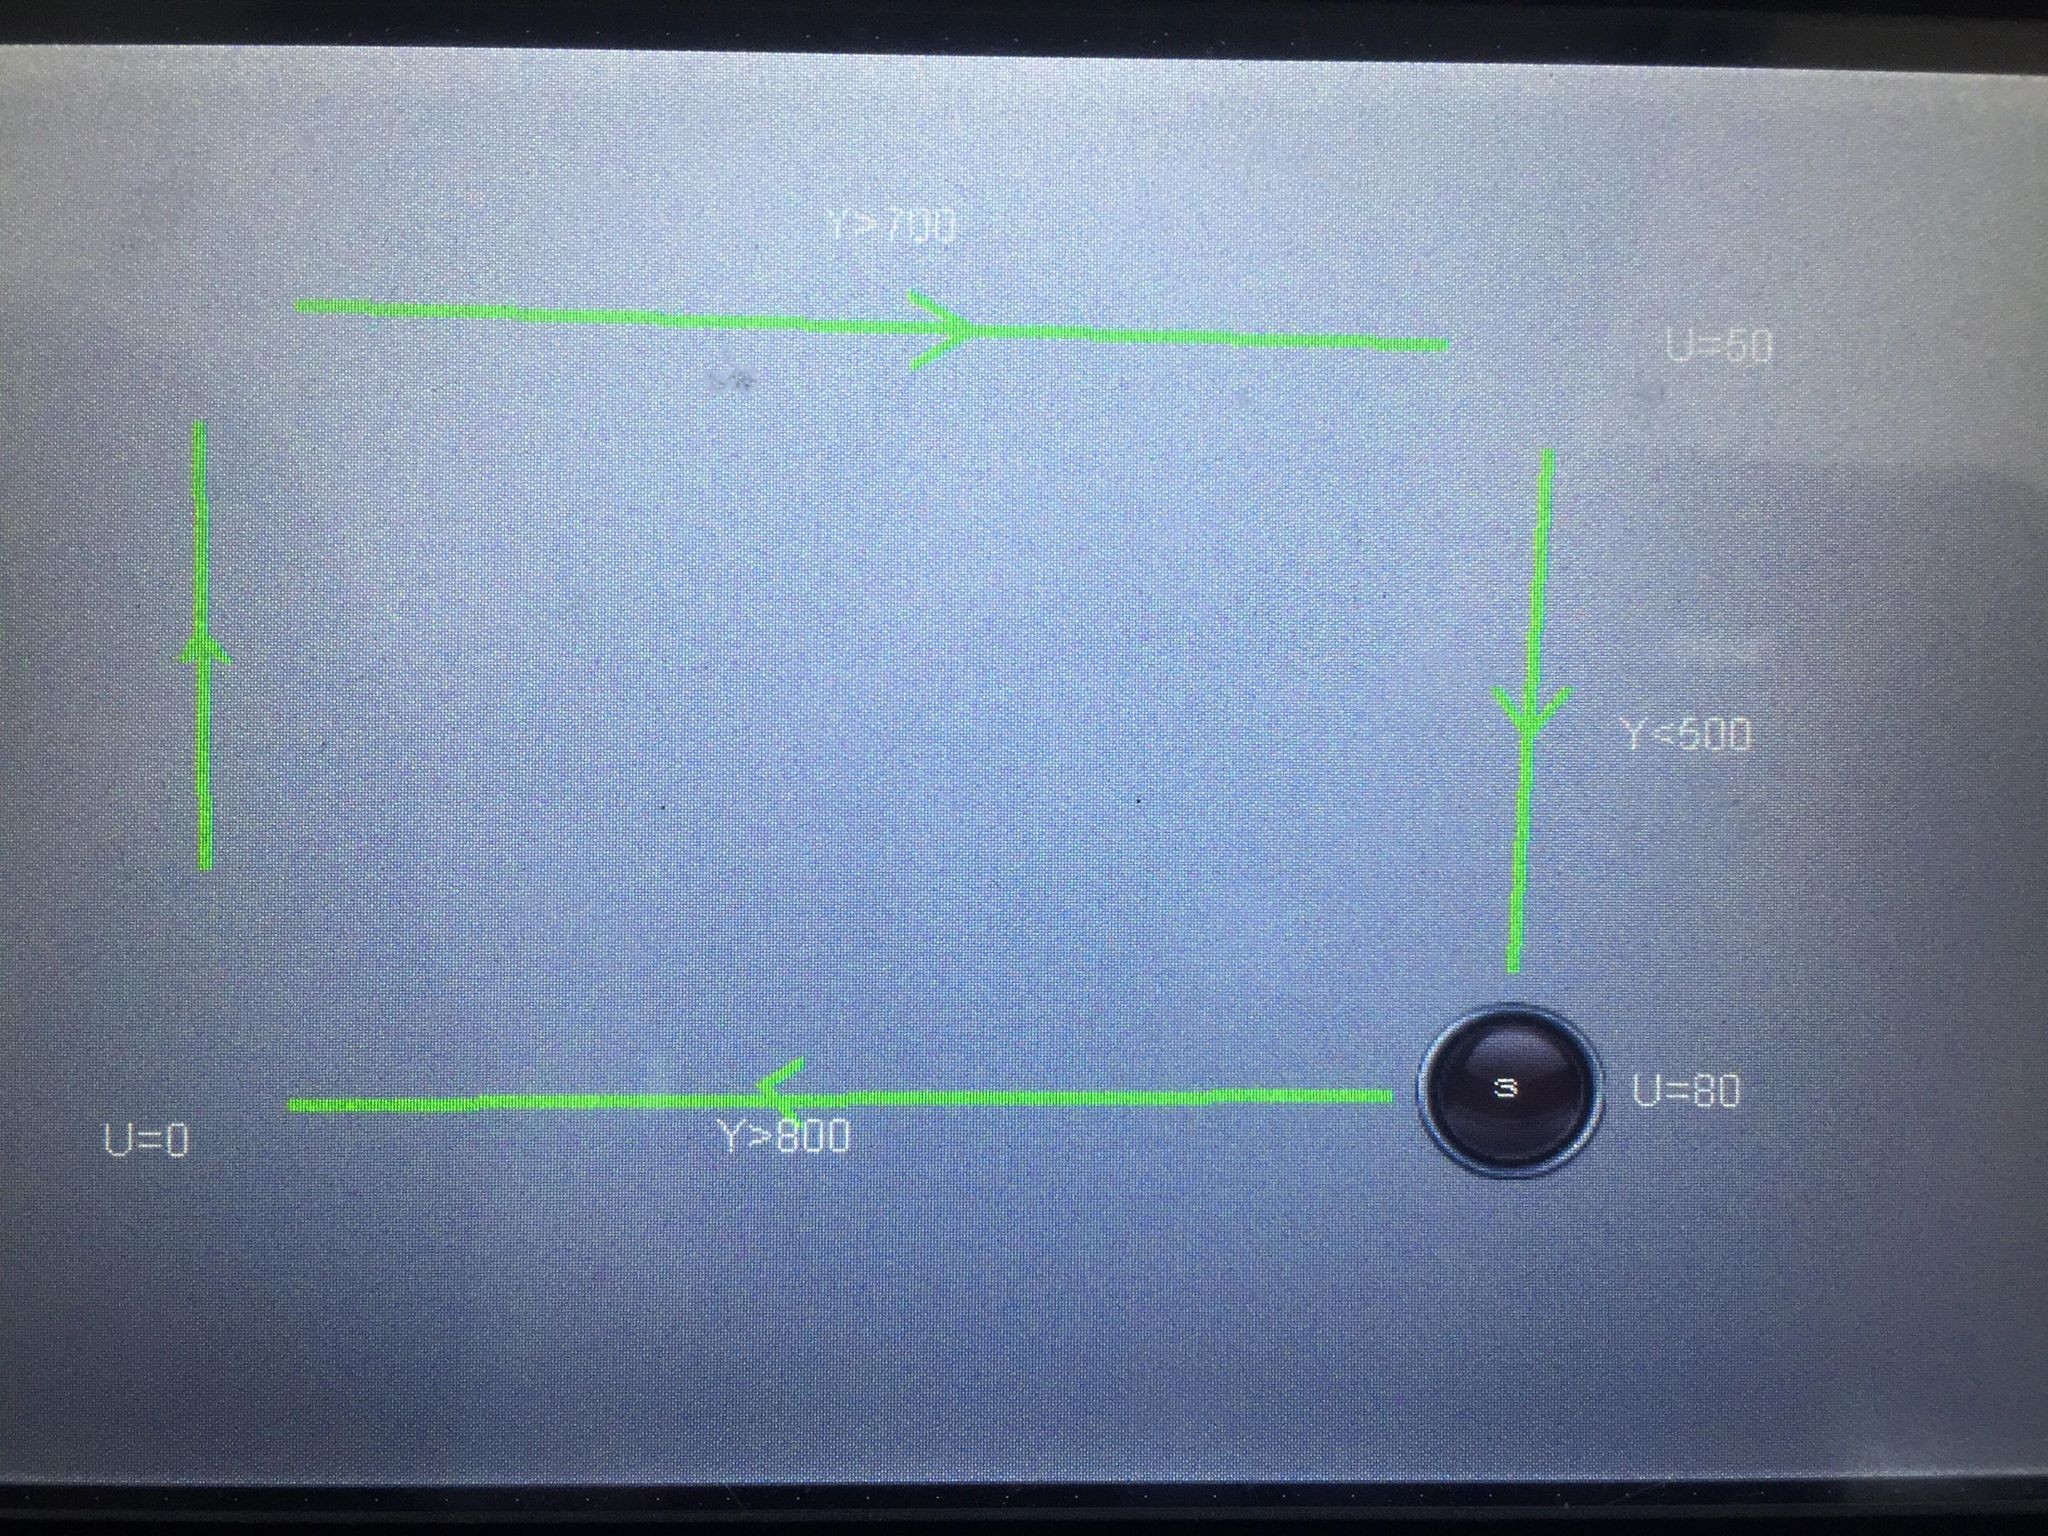
\includegraphics[scale=0.15]{./sections/inteco/images/automat3.jpg}
    \caption{Stan 3. procesu}
\end{figure}

\begin{figure}[H]
    \label{automat_4}
    \centering
    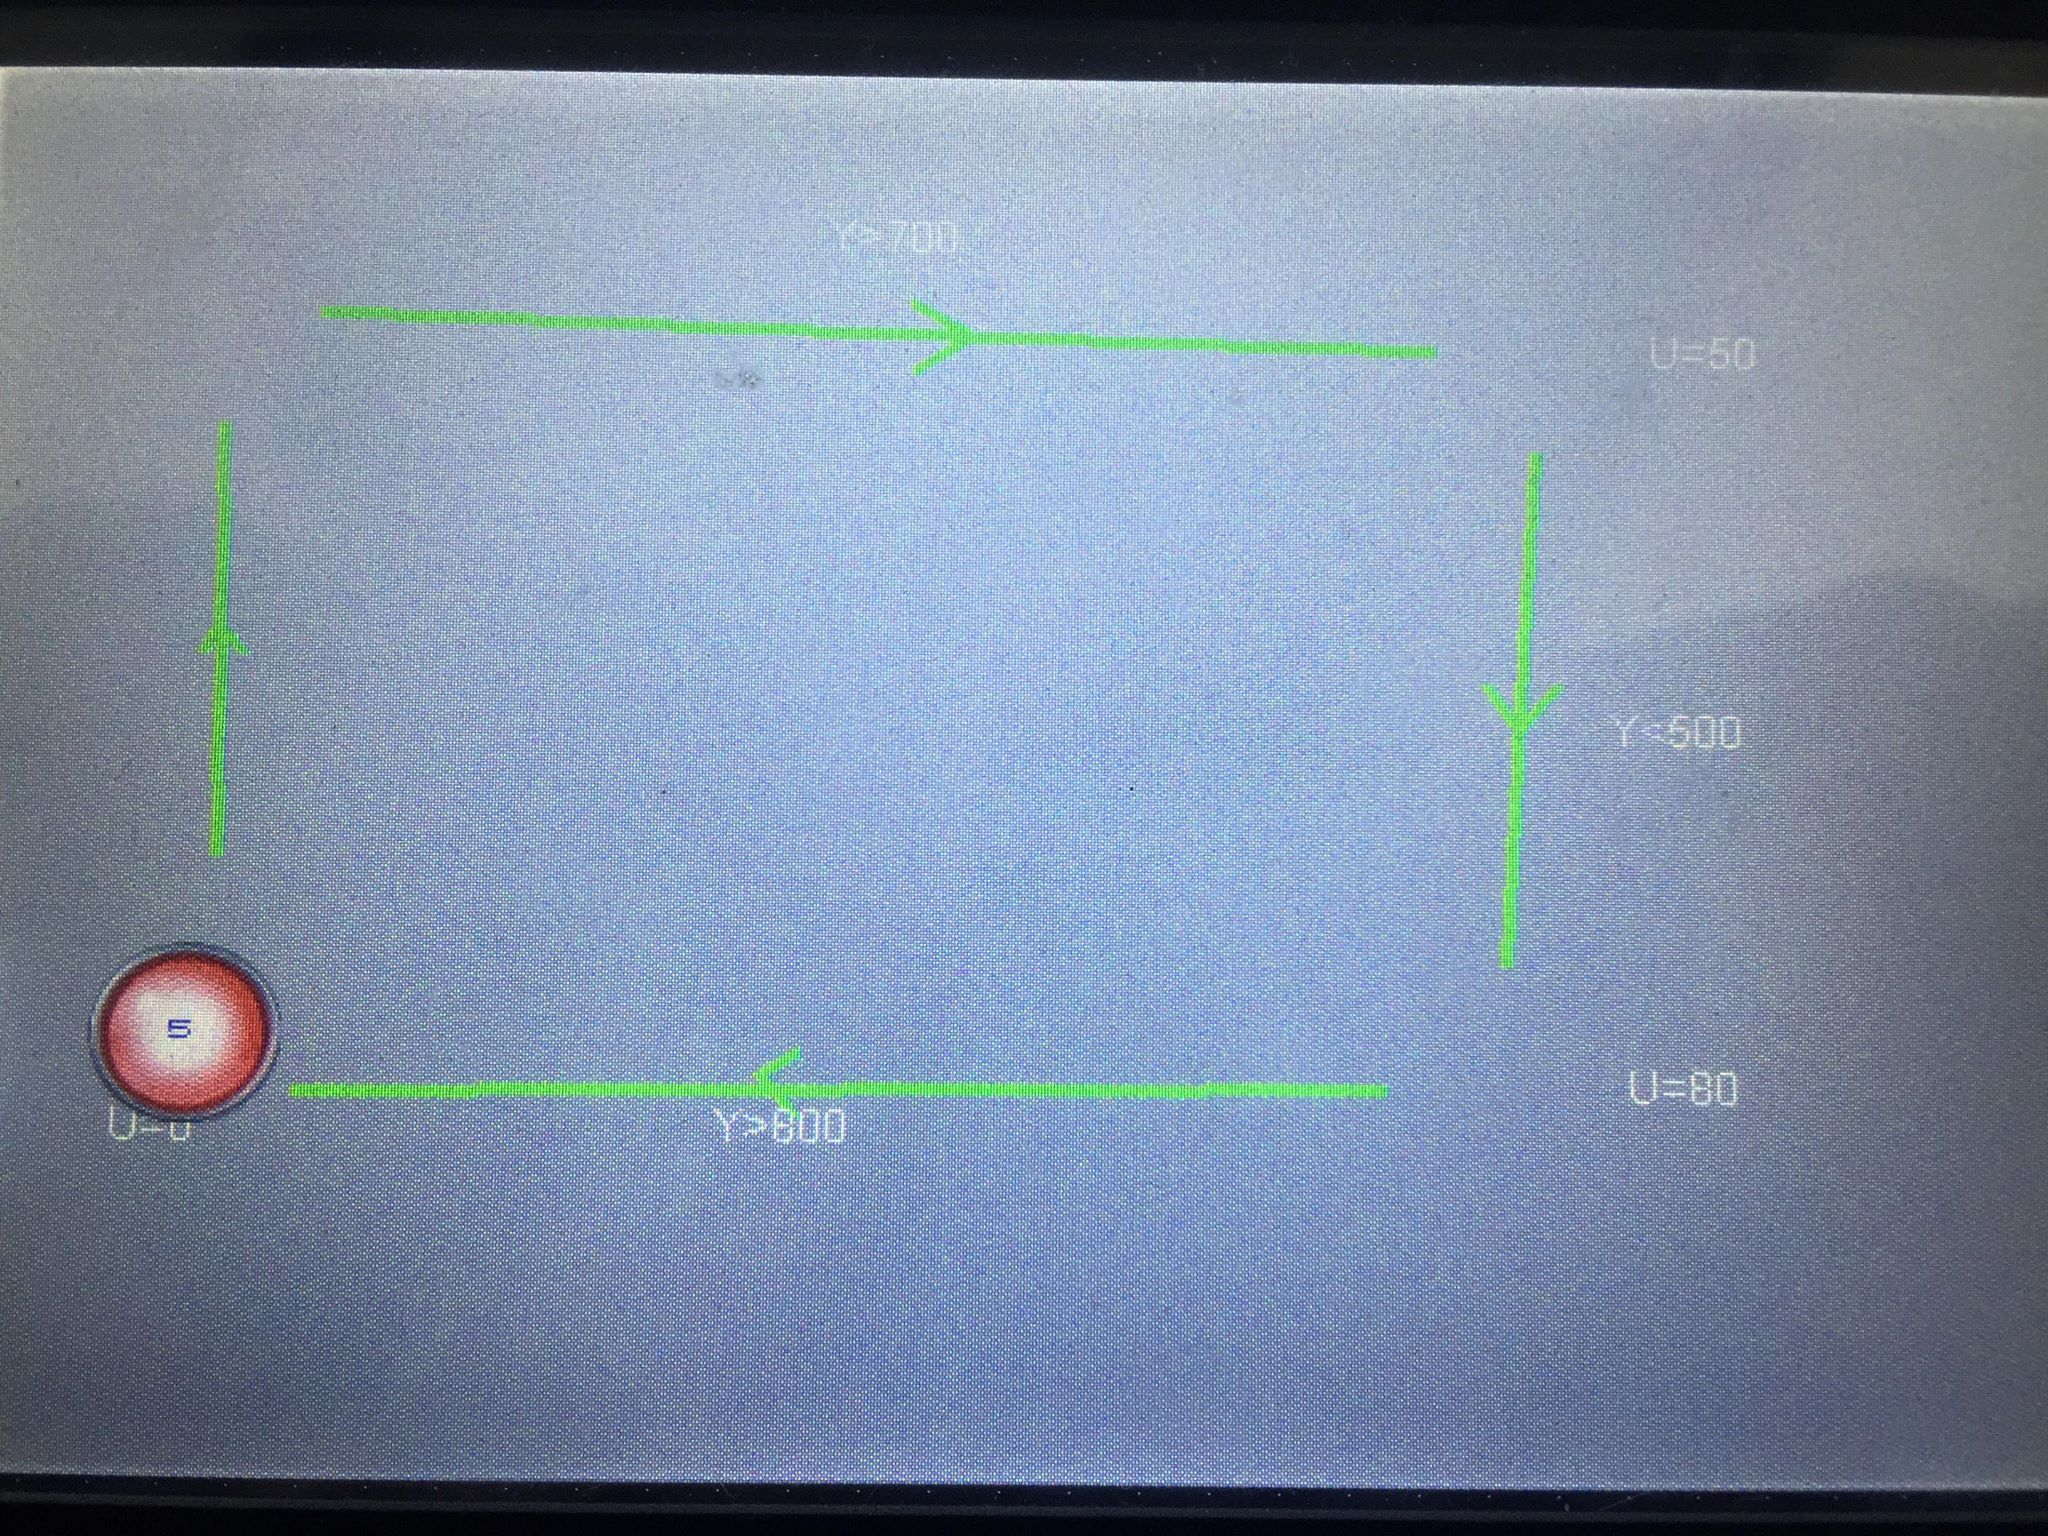
\includegraphics[scale=0.15]{./sections/inteco/images/automat5.jpg}
    \caption{Stan 4. procesu}
\end{figure}


